\chapter{Entwurf}
\thispagestyle{standard}
\pagestyle{standard}
\renewcommand{\footrulewidth}{0.4pt}
\lfoot{\small Refik Kerimi}

In diesem Kapitel werden die Muster und die Anforderungen bzw. die Umsetzung der \acl{PWA}en (\acs{PWA}) im Allgemeinen betrachtet.


\section{Übersicht PWA}\label{sub:Übersicht PWA}
%https://developers.google.com/web/ilt/pwa/introduction-to-progressive-web-app-architectures
% Die Architektur soll beschrieben weden
Im Gegensatz zur \acl{NA} (\acs{NA}) ist die \acl{PWA} (\acs{PWA}) eine \acl{SC} (\acs{SC}) Architektur, diese wird nicht auf dem Client gespeichert sondern es wird über den Browser und das HTTPS-Protokoll zwischen Client und Server kommuniziert. Im Unterschied zu HTTP ist, wie in Abbildung \ref{fig:HTTP_HTTPS} zu sehen, die Verbindung verschlüsselt.

\begin{figure}[h]
	\centering
	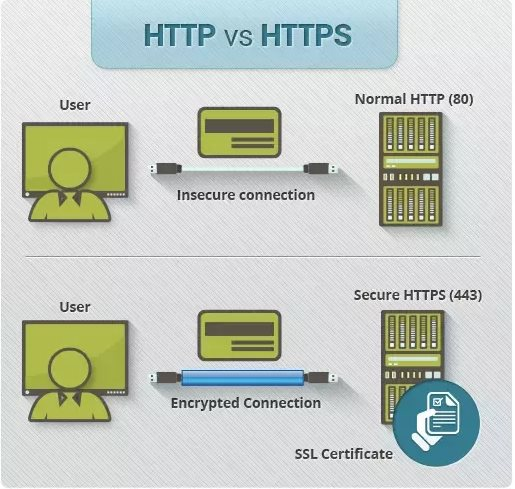
\includegraphics[width=6cm]{BilderAllgemein/HTTP_HTTPS}\medskip
	\caption{Unterschied HTTP/HTTPS \cite{HTTPS}}
	\label{fig:HTTP_HTTPS}
\end{figure}

Dies hat den Vorteil das die Applikation sowie die Updates wie schon in Kapitel \ref{chap:PWAvs.NativeApplikationvsWeb Applikation} erwähnt nicht downgeloaded und installiert werden müssen, das wird alles Server seitig erledigt. 

\newpage




